\documentclass[aspectratio=169]{beamer}
\usepackage[english]{babel}
\usepackage{amsmath,amsfonts}
\usepackage{multicol}

\usepackage{IEEEtrantools}
\usepackage{multirow}
% beamer setup

%\usecolortheme{dove}

\setbeamertemplate{navigation symbols}{}
\setbeamertemplate{itemize items}[ball]

\usepackage{tikz}
\usetikzlibrary{shapes,arrows}
\usetikzlibrary{positioning}
\tikzstyle{block} = [rectangle, draw, rounded corners]
\tikzstyle{line} = [draw, -latex']

\DeclareMathOperator*{\argmin}{argmin}
\DeclareMathOperator*{\argmax}{argmax}
\DeclareMathOperator{\E}{\mathbb{E}}
\DeclareMathOperator{\I}{\mathbb{I}}

\AtBeginSection[]{
  \begin{frame}[plain]
  \addtocounter{framenumber}{-1}
  \vfill
  \centering
  %\begin{beamercolorbox}[sep=8pt,center,shadow=true,rounded=true]{title}
    %\usebeamerfont{title}
    \Huge{\insertsectionhead\par}%
  %\end{beamercolorbox}
  \vfill
  \end{frame}
}


\newcommand{\backupbegin}{
   \newcounter{framenumberappendix}
   \setcounter{framenumberappendix}{\value{framenumber}}
}
\newcommand{\backupend}{
   \addtocounter{framenumberappendix}{-\value{framenumber}}
   \addtocounter{framenumber}{\value{framenumberappendix}} 
}




\title{The Economics of Shotgun Marriage}
\subtitle{and Household Bargaining}
\author{Egor Kozlov}

\institute{
  Department of Economics\\
  Northwestern University}
  
  
\setbeamertemplate{footline}[frame number]

  
%  \usepackage{pgf}
%\logo{\pgfputat{\pgfxy(0,0)}{\pgfbox[right,base]{\footnotesize{\insertframenumber\,/\,\inserttotalframenumber}}}}
%\newcommand{\nologo}{\setbeamertemplate{logo}{}}

\let\olditem\item
\renewcommand{\item}{%
\olditem\vspace{\fill}} 

\begin{document}



\begin{frame}[plain]
\addtocounter{framenumber}{-1}
\date{\scriptsize}
\titlepage
\end{frame}


\begin{frame}
\frametitle{Two-Parent Family Is A Choice}

\textbf{Shotgun marriage} --- marriage that happens soon after a woman gets pregnant.
% many, much less stable, worse among the educated. pt is economics how they get formed, how do the
\begin{itemize}
\item Around 1/4 couples in the US have kids \textbf{before} or \textbf{at the year} of their marriage
\item These marriages are significantly less stable, especially among \textbf{educated people} % marginal marriage
\item Both social norms and economics are expected to drive this
%\item Especially less stable among \textbf{more educated and adult}%(college: 6\% single mothers, 4\% in shotgun marriages)
\item Overall, they contribute to creation of single mothers and blended families
% college grads: 4% in KF marriages and 4% are single mothers
% high school grads: 11% in KF marriages and 20% are single mothers
\end{itemize}
\end{frame}


%
%\begin{frame}
%\frametitle{Questions}
%\begin{itemize}
%\item Drivers of inequality:
%\begin{itemize}
%\item Focusing on unmarried young single mothers omits an important transition
%\item Unplanned pregnancies look different between age and education groups
%\item Divorced parents may be worse than never married
%\end{itemize}
%\item Value of marriage:
%\begin{itemize}
%\item Do pregnancies trigger marriages? If so, why?
%\item If shotgun marriage is risky, why people agree?
%\end{itemize}
%\end{itemize}
%
%\end{frame}


\begin{frame}
\frametitle{Roadmap}
\begin{enumerate}
\item Document the shotgun marriage and its outcomes empirically
\item Use these empirical relations to estimate a model capturing:
\begin{itemize}
\item limited commitment in marriage
\item lifecycle, income and savings
\item fertility and child expenditures
\end{itemize}
\item Look at what drives the difference in marriage performance
\begin{itemize}
\item what explains the education gradient?
\item should policies bother to fix the difference?
\item what is the value of marriage in general?
\end{itemize}
\end{enumerate}
\end{frame}

\begin{frame}
\frametitle{Summary of Results}
\begin{itemize}
\item 23\% of women had the first child before their first marriage (kids first)
\item They are 1.8 times more likely to be divorced than ``marriage first''
%\item College grads: 2.8 times more likely to be divorced
%\begin{itemize}
%\item though smaller kids first share (just 10\%)
%\end{itemize}
\item My structural model corrects selection and data imperfections
\item Model answers:
\begin{itemize}
%\item Causal content: kids first people divorce X times more
\item Social stigma explains 40\%--50\% of the divorce differences for college people
\item Expensive childcare explains the rest
\item Stigma matters less for high school graduates
\end{itemize}
\end{itemize}
\end{frame}


\begin{frame}
\frametitle{Literature}
\begin{itemize}
\item Empirical literature documents the scope of shotgun marriage around the world:
\begin{itemize}
\item Gibson-Davis et al (2016), Guzzo (2009),  Nuevo-Chiquero (2014)
\item Mostly descriptive
\end{itemize}
\item Dynamic limited commitment models of divorce and marriage:
\begin{itemize}
\item Marcet, Marimon (2019), Mazzocco (2007) --- setting up the framework
\item Voena (2015), Shephard (2019); Lafortune, Low  (2019) --- applied questions
\item Mostly ignore or simplify interaction with fertility
\end{itemize}
\item Unplanned and teenage pregnancy literature:
\begin{itemize}
\item Ejrnæs, Jørgensen (2018) --- lifecycle model
\item Card, Wise (1978) to Ashcraft et al (2013) --- lots of empirical papers
\item Treat household structure as fixed or exogenous
\end{itemize}
\end{itemize}
\end{frame}




\section{Data}
\begin{frame}
\frametitle{Sources: ACS 2009--2015 and others}
\begin{itemize}
\item Main exercises and model estimation are done on American Community Survey
\item Huge sample size and enough information to show many things 
\item Individual marriage and fertility history are observed partially
\begin{itemize}
\item Only the most recent marriage date --- restrict to ``married once'' when matters
\item Pick age $\in [21,40]$ to have good information on fertility
\end{itemize}
\item Smaller datasets with better histories for robustness and extra evidence:
\begin{itemize}
\item SIPP, NSFG, NSFH --- all have similar patterns
\end{itemize}
\end{itemize}
\end{frame}

\begin{frame}[label=kfandmf]
\frametitle{Kids First and Marriage First}
\[\Delta T = \text{Year The First Child Born} - \text{Year The First Marriage Happened}.\]
\begin{itemize}
\item Marriage First \textbf{(MF)}: $\Delta T \in \{1,2,...\}$ (kids at least at the next year)
\item Kids First \textbf{(KF)}: $\Delta T \in \{...,-2,-1,0\}$ (shotgun marriage in a wide sense)
\item Not a full partition%: at 30 only 31\% on the US women have kids and exactly one marriage
\item Most of the comparisons are within this group
\end{itemize}
\hyperlink{extra-restrictions}{\beamerbutton{Extra Restrictions}} 
\end{frame}

\begin{frame}[label=dt_graph]
\frametitle{Kids First Women Are Divorced More Often: Key Graph}
\begin{center}
\includegraphics[scale=0.75]{div_5y_by_dt.pdf}
\end{center}
\vspace{-1cm}
\hyperlink{dt_graph_educ}{\beamerbutton{by education}} 
\end{frame}


\begin{frame}
\frametitle{Kids First Women Are Divorced More Often: Quantification}
\begin{center}
\begin{tabular}{l c c c c c}\hline
& &  \multicolumn{2}{c}{\small \% divorced if ...} \\
& \% KF & MF & KF & \% diff &  Ratio \\\hline
\multicolumn{6}{c}{\textit{Cross-Section: All Females 21--40 married once}}\\
All females & 23.2 &  10.2 & 18.1 & 7.9 & 1.77  \\
College & 10.0 & 5.4 & 14.8 & 9.4 & 2.76 \\
High school & 34.3 & 13.9 & 17.3 & 3.3 & 1.24 \\\hline
\multicolumn{6}{c}{\textit{Controlling strategies}}\\\hline
%\multicolumn{2}{l}{College 5 y after marriage} & 5.1 & 14.3 & 9.2 & 2.79 \\
\multicolumn{4}{l}{Regression with controls}   & 7.0 & 1.69 \\
\multicolumn{4}{l}{Regression with controls + income}   & 6.1 & 1.60 \\\hline
\multicolumn{6}{p{0.7\linewidth}}{\footnotesize Regression: $\text{Divorced}_i = \Delta \cdot \text{KF}_i + X_i\gamma + \varepsilon_i$ (if $\text{KF}_i = 1$ or $\text{MF}_i = 1$)}\\
\multicolumn{6}{p{0.7\linewidth}}{\footnotesize Controls are two-way FE for interactions of age with education, time since marriage, time since birth, and one-way FE for geography, race, survey year. 
Income is 3rd degree polynomial of log per-hour reported income for working $\geq 10$ hours per week and earning $\geq \$3000$ per year.
}\\
\multicolumn{6}{p{0.7\linewidth}}{\footnotesize Data: American Community Survey 2009--2016.}\\\hline
\end{tabular}
\end{center}
\end{frame}

\begin{frame}
\frametitle{Kids First Women Are Divorced More Often: Robustness \& Extra}
\begin{itemize}
\item SIPP exercise: smaller sample but full marital history and fertility history
\begin{itemize}
\item Similar ratios with larger magnitudes when include remarried people
\end{itemize}
\item Duration model: NSFH, historic data from 80s
\begin{itemize}
\item Hazard ratio of 1.45, college: 2.23
\end{itemize}
\item More details: NSFG, 2015--2017 data
\begin{itemize}
\item KF: 30\% true shotgun, 50\% marry after birth, 20\% marry new partner
\item True shotgun have the highest share of divorced
\end{itemize}
\end{itemize}
\end{frame}
%
%
%\begin{frame}
%\frametitle{Need For The Model}
%\begin{enumerate}
%\item Observables provide limited information. Missing things: relationship quality, potential partners, future divorces
%\item Data are not perfect. Limited histories, unobservable income if out of labor force, step or own children
%\end{enumerate}
%\end{frame}



\section{Model}
\begin{frame}
\frametitle{Summary: Lifecycle, Fertility, Divorce}
\begin{itemize}
\item Lifecycle model with finite horizon
\item People are heterogeneous with respect to age $t$, wages $w$ and savings $a$
\item Couples also differ by relationship quality $\psi$ and spouses' decision power $\theta$
\item Fertility: endogenous decision to have a child (just one) + shocks
\item Limited commitment: decisions are affected by outside options of divorce
\end{itemize}
\end{frame}



\begin{frame}
\frametitle{Modeling Shotgun Marriage}
\begin{center}
\vspace{-0.2cm}
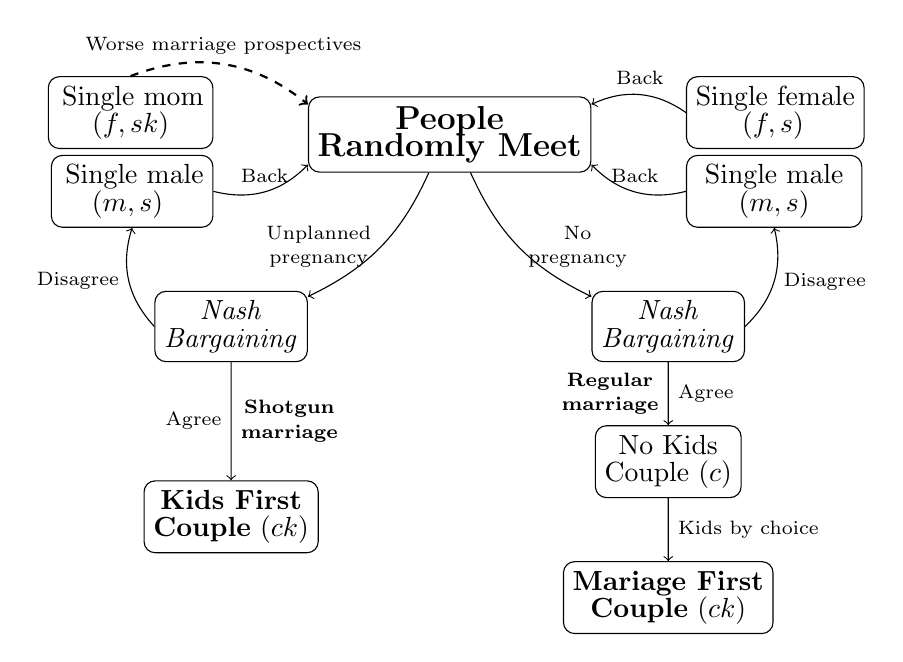
\begin{tikzpicture}[every text node part/.style={align=center}, scale=0.75]
   % Place nodes
   \node [block] (1) {\large \textbf{People}  \\[-0.5ex]  \large  \textbf{Randomly Meet}};
   \node [block, below left = 1.5 cm and 0.0 cm of 1] (2) {\textit{Nash} \\[-0.5ex] \textit{Bargaining}};   
   \node [block, below right = 1.5 cm and 0.0 cm of 1] (3) {\textit{Nash} \\[-0.5ex] \textit{Bargaining}};   

   \node [block, below = 1.5 cm of 2] (5) {\textbf{Kids First} \\[-0.5ex] \textbf{Couple} ($ck$)};
   \node [block, below = 0.8 cm of 3] (7) {No Kids \\[-0.5ex] Couple ($c$)};
   \node [block, below = 0.8 cm of 7] (8) {\textbf{Mariage First} \\[-0.5ex] \textbf{Couple} ($ck$)};
   \draw[->] (1) to [bend left = 20] node [left] {\scriptsize Unplanned \\[-0.75ex] \scriptsize pregnancy} (2);
   \draw[->] (1) to [bend right = 20] node [right] {\scriptsize No \\[-0.75ex] \scriptsize pregnancy} (3);
   \draw[->] (2) to node [left] {\scriptsize Agree} node [right] {\scriptsize \textbf{Shotgun} \\[-0.75ex]  \scriptsize \textbf{marriage}} (5);
   \draw[->] (3) to node [right] {\scriptsize Agree} node [left]  {\scriptsize \textbf{Regular} \\[-0.75ex]  \scriptsize \textbf{marriage}} (7);
   \draw[->] (7) to node [right] {\scriptsize Kids by choice} (8);   
    \node [block, above left   = 0.8 cm and -0.75 cm of 2] (4) {\,Single male \\[-0.5ex] ($m,s$)\,\,};
    \node [block, above left   = 1.8 cm and -0.75 cm of 2] (4-sm) {\,Single mom \\[-0.5ex]  ($f,sk$)};
	\node [block, above right   = 0.8 cm and -0.75 cm of 3] (6) {\,\,Single male\,\,\\[-0.5ex] ($m,s$)};
    \node [block, above right   = 1.8 cm and -0.75 cm of 3] (6-f) {Single female\\[-0.5ex] ($f,s$)\,};   
    \draw[->] (2.180) to [bend left = 30] node [left] {\scriptsize Disagree} (4.270);
    \draw[->] (3.0) to [bend right = 30] node [right] {\scriptsize Disagree} (6.270);
     \draw[->] (6.180) to [bend left = 30] node [above] {\scriptsize Back}  (1.-12);
   \draw[->] (6-f.180) to [bend right = 30] node [above] {\scriptsize Back} (1.12);
   \draw[->,thick,dashed] (4-sm.90) to [bend left = 30] node [above] {\scriptsize Worse marriage prospectives}  (1.168);
   \draw[->] (4.0) to [bend right = 30] node [above] {\scriptsize Back} (1.192);
   
   
\end{tikzpicture}
\end{center}
\end{frame}


\begin{frame}
\frametitle{Value Function: Female, Single}
\framesubtitle{$p^m_t$ --- probability of meeting, $p^p_t$ --- probability of unplanned pregnancy, $m_t$ --- agree to marry}
\begin{align*}
V^{f,s}_t(a,w) = \max\limits_{c,a'} \Bigg\{ \frac{c^{1-\sigma}}{1-\sigma} + \beta \cdot \E_t \Big\{  & 
%& \\ \text{ (did not meet anyone): \ } & 
(1-p^{\text{m}}_t)\cdot V_{t+1}^{f,s}(a',w') \\
\text{ \footnotesize (met and not pregnant): \ }& +  p^{\text{m}}_t\cdot (1- p^{p}_t) \cdot \left[ m^{np}_t \cdot V^{f,c}_{t+1}  + (1-m^{np}_t)\cdot  V^{f,s}_{t+1}\right] \\
\text{ \footnotesize (met and pregnant): \ } & + p^{\text{m}}_t \cdot p^{\text{p}}_t\cdot   \left[ m^p_t \cdot V^{f,ck}_{t+1}  + (1-m^p_t)\cdot  V^{f,sk}_{t+1}\right] \Big\} \Bigg\} \\
\text{ \footnotesize (budget constraint): \ } & c + a' = R\cdot a  + w , \\
\text{ \footnotesize (wage evolution): \ } & \log w = z + \text{Trend}_t, \ \ z' = z + \varepsilon^{f}.
\end{align*}
\end{frame}


\begin{frame}
\frametitle{Value Function: Couple, No Children}
\framesubtitle{$k_t$ --- give a birth, $d_t$ --- get a divorce, $\tilde{V}$ --- values at divorce}
\begin{align*}
V^{c}_t(a,w_f,w_m,\psi,\theta) = \max\limits_{c_f,c_m,a',k} \Bigg\{ & \theta^f \cdot \frac{c_f^{1-\sigma}}{{1-\sigma}}  + \theta^m \cdot \frac{c_m^{1-\sigma}}{1-\sigma}  + \psi + \beta \cdot \E_t \Big\{   \\
\text{ \footnotesize (stay, no birth): \ } & + (1-d_t) \cdot (1-k_t) \cdot  \left[ \theta^f \cdot  V^{f,c}_{t+1} + \theta^m \cdot V^{m,c}_{t+1}  \right] \\
\text{ \footnotesize (stay, give a birth): \ } &  + (1-d_t) \cdot k_t \cdot  \left[ \theta^f \cdot  V^{f,ck}_{t+1} + \theta^m \cdot V^{m,ck}_{t+1}  \right]  \\
\text{ \footnotesize (divorce): \ } & + d_t  \left[ \theta^f \cdot  \tilde{V}^{f,s}_{t+1} + \theta^m \cdot \tilde{V}^{m,s}_{t+1}  \right]  \Big\} \Bigg\}\\
\text{ \footnotesize (budget constraint): \ } &{\normalsize \left[c_f^{1+\rho} + c_m^{1+\rho}\right]^{\frac1{1+\rho}} + a' = R\cdot a + w_f + w_m}\\
\text{ \footnotesize (match quality evolution): \ } &{\normalsize \psi' = \psi + \varepsilon^{\psi}}\\
\text{ \footnotesize \textbf{(participation constraints)}: \ } &{\normalsize V^{f,c\bullet}_{t+1} (\cdots,\theta') \geq \tilde{V}^{f,s}_{t+1}, \ \ V^{m,c\bullet}_{t+1} (\cdots,\theta') \geq \tilde{V}^{m,s}_{t+1}.}\\
\end{align*}
\end{frame}


\begin{frame}
\frametitle{Value Function: Couple and Child}
\framesubtitle{$d_t$ --- get a divorce, $\tilde{V}$ --- values at divorce}
\begin{align*}
V^{ck}_t(a,w_f,w_m,\psi,\theta) = \max\limits_{c_f,c_m,x,l_f,a'} \Bigg\{ & \theta^f \cdot \frac{c_f^{1-\sigma}}{{1-\sigma}}  + \theta^m \cdot \frac{c_m^{1-\sigma}}{1-\sigma}  + \psi + \\ \text{ \footnotesize (child is a public good): \ }  & \phi + \alpha \cdot \frac{Q^{1-\sigma}}{1-\sigma} +  \beta \cdot \E_t \Big\{   \\
\text{ \footnotesize (stay): \ } & + (1-d_t) \cdot  \left[ \theta^f \cdot  V^{f,ck}_{t+1} + \theta^m \cdot V^{m,ck}_{t+1}  \right] \\
\text{ \footnotesize (divorce): \ } & + d_t  \left[ \theta^f \cdot  \tilde V^{f,sk}_{t+1} + \theta^m \cdot \tilde V^{m,s}_{t+1}  \right]  \Big\} \Bigg\}\\
\text{ \footnotesize (budget constraint): \ } &{\normalsize \left[c_f^{1+\rho} + c_m^{1+\rho}\right]^{\frac1{1+\rho}} + x + a' = R\cdot a + w_f\cdot l_f + w_m}\\
\text{ \footnotesize (child quality flow): \ } &{\normalsize Q = \left[x^\lambda + \kappa \cdot (1-l_f)^\lambda\right]^{\frac1\lambda}, \ \ \ Q\geq \bar{Q}} \text{ \footnotesize  (subsistence constraint) } \\
\text{ \footnotesize (female skills depreciate): \ } &{\normalsize \log w_f = z_f + \text{Trend}_{f,t}, \ \ z'_f = z_f + \varepsilon^f - \delta(l^f)}\\
\end{align*}
\end{frame}



\begin{frame}
\frametitle{Renegotiation and Divorce}
\framesubtitle{Are generated by the participation constraints}
\begin{itemize}
\item Bargaining weights $\theta$ adjust to satisfy both participation constraints.
\item If no adjustment is possible, the couple divorces
\item Assets are split evenly upon divorce
\item If couple with a child divorces wife becomes a single mother
\item Child support: adjustment in permanent income component $z$
\end{itemize}
\end{frame}

\begin{frame}
\frametitle{Marriage}
\begin{itemize}
\item Singles meet singles with similar $a$ and $z$ 
\item Potential couple gets a draw of match quality $\psi$
\item If both partners agree to marry, initial $\theta$ is set by symmetric Nash Bargainig
\item Two utility shifters:
\begin{itemize}
\item If unplanned pregnancy happens, partners face social stigma $\phi_s$ if refuse to marry
\item If male meets a single mother, he lose $\phi_m$ for having step children
\end{itemize}
\end{itemize}
\begin{center}
{\footnotesize
\begin{tabular}{|l||c|c||c|c||c|}\hline
 & \multicolumn{2}{|c||}{Male gets:} & \multicolumn{2}{|c||}{Female gets:} \\\hline
Situation & Agree & Disagree & Agree & Disagree \\\hline
Regular match & $V^{m,c}_t(\theta)$ & $V^{m,s}_t$ & $V^{f,c}_t(\theta)$ & $V^{f,s}_t$ \\
Unplanned pregnancy & $V^{m,ck}_t(\theta)$ & $V^{m,s}_t - \phi_s$ & $V^{f,ck}_t(\theta)$ & $V^{f,s}_t - \phi_s$ \\
Meeting a single mother & $V^{m,ck}_t(\theta) - \phi_m$ & $V^{m,s}_t$ & $V^{f,ck}_t(\theta)$ & $V^{f,s}_t$ \\\hline
\end{tabular}
}
\end{center}
\end{frame}

\section{Mechanics}
\begin{frame}
\frametitle{Unplanned Pregnancy $\Rightarrow$ Worse Match?}
\framesubtitle{Model Implications}

\begin{itemize}
\item Women enter the shotgun marriages because:
\begin{itemize}
\item Child costs need to be shared (returns to scale)
\item Finding a new partner is trickier once you have a child
\end{itemize}
\item Men enter the shotgun marriage because:
\begin{itemize}
\item They like their kids and lose access to them otherwise
\end{itemize}
\item Even with a good match, mistimed pregnancy is a risk
\item Scope of these effects depend on exact calibration
\end{itemize}
\end{frame}


\begin{frame}
\frametitle{Unplanned Pregnancy $\Rightarrow$ Women Lose a Lot, Men Gain a Little}
\framesubtitle{Nash Bargaining Surplus: $NBS(\theta) = (V^{f,\text{agree}}(\theta) - V^{f,\text{disagree}})\times(V^{m,\text{agree}}(\theta) - V^{m,\text{disagree}})$}
\begin{center}
\includegraphics[scale=0.7]{change_upp.pdf}
\end{center}

\end{frame}

\begin{frame}
\frametitle{...Hence Less Picky Partners + Lower Female Decision Power}
\begin{center}
\begin{tabular}{c c}
\hspace{-1cm} \includegraphics[scale=0.5]{barg_reg_match.pdf} & \includegraphics[scale=0.5]{barg_upp.pdf}
\end{tabular}
\end{center}
Social stigma $\approx$ draw $\psi$ from different distribution if pregnant.  %More productive women suffer more.
\end{frame}


\section{Fit and Results}

\begin{frame}
\frametitle{Too Much Heterogeneity}
\begin{itemize}
\item College and non-college people have very distinct patterns
\item They cannot be summarized well with one-dimensional productivity
\item Therefore I focus on two subsamples:
\begin{itemize}
\item High education: bachelor degree or more
\item Low education: high school or less
\end{itemize}
\item \textbf{Today:} estimates for high education (large impact of unplanned pregnancy)% + preliminary comparison with low education
\end{itemize}
\end{frame}

\begin{frame}
\frametitle{Targets}
\begin{tabular}{l p{0.5\linewidth}}\hline
\multicolumn{1}{l}{Target} & \multicolumn{1}{l}{Informative about} \\\hline
\footnotesize \% with kids 1--10 years after marriage & \footnotesize  Fertility parameters: $\phi$, $\alpha$ \\
\footnotesize \% MF females in population at 23--35 & \footnotesize  $\phi$, $\alpha$ + meeting probabilities \\
\footnotesize \% KF females in population at 23--35 &\footnotesize   meeting + unplanned preg probabilities\\
\footnotesize \% never married with and without kids at 23--35 & \footnotesize  meeting + unplanned preg probabilities + $\phi_r$\\
\footnotesize \% divorced with and without kids at 23--35 & \footnotesize  distribution of $\psi$ + fertility parameters + $\phi_r$ \\
\footnotesize child expenditures share, \% in LF with kids & \footnotesize  household technology: $\kappa$, $\alpha$ and $\bar{Q}$ \\
\footnotesize \% divorced 1--10 years after marriage if KF or MF & \footnotesize  social stigma, $\bar{Q}$ and more ... \\\hline
\end{tabular}
\end{frame}



\begin{frame}
\frametitle{Data}
\framesubtitle{High school in red, college in black}
\begin{center}
\begin{tabular}{c c}
\hspace{-0.5cm} \includegraphics[scale=0.33]{div_kfmf_dc.pdf} & \includegraphics[scale=0.33]{popshares_dc.pdf} \\
\hspace{-0.5cm} \includegraphics[scale=0.33]{evermar_dc.pdf} & \includegraphics[scale=0.33]{everkids_dc.pdf} \\
\end{tabular}
\end{center}
\end{frame}


\begin{frame}
\frametitle{Estimates}
\framesubtitle{Simulated Method of Moments (SMM) with optimization routine from Arnoud et al, 2019; 14 parameters}
\begin{tabular}{l c c c}\hline
& High Education & Low Education & Source \\\hline
\multicolumn{4}{c}{Utility from kids: $\phi + \alpha \cdot \frac{Q^{1-\xi}}{1-\xi}$, \ $Q = [x^{\lambda} + \kappa\cdot(1-l_f)^{\lambda}]^{\frac1{\lambda}}$. $Q\geq \bar{Q}$}\\\hline
$\phi$, $\alpha$, $\kappa$  \footnotesize (utility params) &\footnotesize  $(0.96, 0.38, 0.90)$ &\footnotesize $(1.89,0.46, 0.85)$ & SMM \\
$\bar{Q}$ \footnotesize (subsistence constraint) & 0.87 & 0.30 & SMM\\
$\xi$ \footnotesize (power)  & 1.5 & 1.5 & As $\sigma$ \\
$\lambda$ \footnotesize (substitutability)  & 0.7 & 0.7 & \footnotesize Sommer (2016) \\\hline\hline %Attanasio and Weber (1995) \\\hline
%\multicolumn{4}{p{0.9\linewidth}}{\footnotesize \textbf{Identification:} hazards of new children over age, \% with kids by years after marriage}\\\hline\hline
\multicolumn{4}{c}{Meeting probability $p^{\text{meet}}$, pregnancy probability $p^{\text{preg}}$: quadratic polynomials}\\\hline
$p^{\text{meet}}$  \footnotesize at (21,28,35) & \footnotesize $(0.23, 0.67, 0.72)$ & \footnotesize  $(0.49, 0.17, 0.49)$& SMM\\
$p^{\text{preg}}$ \footnotesize  at (21,28,35) & \footnotesize  $(0.06, 0.01, 0.06)$ & \footnotesize  $(0.40, 0.08, 0.52)$ & SMM \\\hline\hline
\multicolumn{4}{c}{Additive utility shifters}\\\hline
$\sigma(\psi_0)$  \footnotesize (match quality initial) & 2.70 & 2.58 & SMM \\
$\sigma(\varepsilon^\psi)$  \footnotesize (match quality shock) & 0.38 & 0.48 & SMM \\
$\phi_s$ \footnotesize  (social stigma) & 0.68 & 1.11 & SMM\\
$\phi_m$ \footnotesize   (single mom remarriage loss) & 14.2 & 20.3 & SMM \\\hline
\end{tabular}
\end{frame}



\begin{frame}
\frametitle{Things Fit Well --- Part 1}
\framesubtitle{High Education Sample}
\begin{center}

\begin{tabular}{c c}
\hspace{-1cm}\includegraphics[scale=0.5]{evermar.pdf} &\hspace{-0.5cm} \includegraphics[scale=0.5]{popshares.pdf} \\
\end{tabular}
\end{center}
\end{frame}


\begin{frame}
\frametitle{Things Fit Well --- Part 2}
\framesubtitle{High Education Sample}
\begin{center}
\begin{tabular}{c c}
\hspace{-1cm}\includegraphics[scale=0.5]{div_kfmf.pdf}  & \hspace{-0.5cm} \includegraphics[scale=0.5]{everkids.pdf} 
\end{tabular}
\end{center}
\end{frame}

%
%\begin{frame}
%\frametitle{Fertility Timing Is Hard To Get}
%\framesubtitle{Need Large Taste Shocks To Get The Results}
%\begin{center}
%\includegraphics[scale=0.75]{kids_yaftmar.pdf} 
%\end{center}
%\end{frame}
%

\begin{frame}
\frametitle{Unplanned Pregnancies Are Large Risk}
\framesubtitle{College women}
\[\text{Definition:} \ \  EV = a^*_t(w) \text{ such that } V_{t}^{f,s,\text{with upp}}(a=a^*,w) = V_{t}^{f,s,\text{no upp}}(a=0,w)\]
\begin{center}
\includegraphics[scale=0.6]{upp_welfare.pdf} 
\end{center}
\end{frame}

\begin{frame}[label=cf]
\frametitle{Counterfactual Exercises}
\begin{itemize}
\item Enforcing 20\% child support (divorced fathers pay) \hyperlink{child_support}{\beamerbutton{pictures}} 
\begin{itemize}
\item Divorced in 10 years if KF: 13.5\% $\to$ 10.7\%.
\item More kids + fewer divorces
\end{itemize}
\item Removing social stigma related to shotgun marriage: setting $\phi_s = 0$ \hyperlink{noss}{\beamerbutton{pictures}} 
\begin{itemize}
\item Divorced in 10 years if KF: 13.5\% $\to$ 9.9\%
\end{itemize}
\item Removing remarriage penalty: setting $\phi_r = 0$ \hyperlink{remarriage_penalty}{\beamerbutton{pictures}} 
\begin{itemize}
\item Divorced in 10 years if KF: 13.5\% $\to$ 12.4\%
\item More kids
\end{itemize}
\item Removing gender pay gap: same trend + variance for men and women \hyperlink{pay_gap}{\beamerbutton{pictures}} 
\begin{itemize}
\item Divorced in 10 years if KF: 13.5\% $\to$ 12.6\%
\item Fewer kids somehow
\end{itemize}
\end{itemize}
\end{frame}



\begin{frame}[label=cf]
\frametitle{Conclusions}
\begin{itemize}
\item Risk of unplanned pregnancies explains the pattern well
\item Men generally win from unexpected kids when commitment is limited, enforcing commitment helps
\item Social stigma explains less than half of the difference
\end{itemize}
\end{frame}





\backupbegin


\begin{frame}[label=child_support]
\frametitle{Enforcing Child Support}
\framesubtitle{Divorced in 10 years if KF: 13.5\% $\to$ 10.7\%. Divorced in cross-section if KF: 9.3\% $\to$ 6.7\%. More kids!}
\begin{center}
\begin{tabular}{c c}
\includegraphics[scale=0.45]{div_kfmf_cs.pdf} & \includegraphics[scale=0.45]{kids_cs.pdf} 
\end{tabular}
\end{center}
Mechanics: divorce $\Rightarrow$ $z^m$ decreases so $w^m$ $\downarrow$ 20\%, $z^f$ increases accordingly.

\hyperlink{cf}{\beamerbutton{back}} 
\end{frame}


\begin{frame}[label=noss]
\frametitle{Removing Social Stigma}
\framesubtitle{Divorced in 10 years if KF: 13.5\% $\to$ 9.9\%. Divorced in cross-section if KF: 9.3\% $\to$ 7.7\%}
\begin{center}
\includegraphics[scale=0.66]{removing_ss.pdf} 
\end{center}
\hyperlink{cf}{\beamerbutton{back}} 
\end{frame}

\begin{frame}[label=remarriage_penalty]
\frametitle{Removing Remarriage Penalty For Single Mothers}
\framesubtitle{Divorced in 10 years if KF: 13.5\% $\to$ 12.4\%. Divorced in cross-section if KF: 9.3\% $\to$ 8.9\% + More Kids}
\begin{center}
\begin{tabular}{c c}
\hspace{-1cm} \includegraphics[scale=0.5]{div_kfmf_no_remar.pdf}  &  \includegraphics[scale=0.5]{ever_kids_no_remar.pdf} 
\end{tabular}
\end{center}
\hyperlink{cf}{\beamerbutton{back}} 
\end{frame}


\begin{frame}[label=pay_gap]
\frametitle{Removing Pay Gap}
\framesubtitle{Divorced in 10 years if KF: 13.5\% $\to$ 12.6\%. Divorced in cross-section if KF: 9.3\% $\to$ 8.8\% + Fewer Kids}
\begin{center}
\begin{tabular}{c c}
\hspace{-1cm} \includegraphics[scale=0.5]{eq_pay.pdf}  &  \includegraphics[scale=0.5]{everkids_eq_pay.pdf} 
\end{tabular}
\end{center}
\hyperlink{cf}{\beamerbutton{back}} 
\end{frame}




\begin{frame}[plain,label=extra-restrictions]
\frametitle{Extra Restrictions}
\begin{itemize}
\item I do not classify as KF or MF people with $\Delta T < -5$ or $\Delta T > 10$
\item I exclude small share of people with marital statuses ``separated'', ``widowed'' and ``spouse absent''
\item This does not affect the results much but helps to ensure consistency
\end{itemize}
\hyperlink{kfandmf}{\beamerbutton{back to KF and MF}} 
\end{frame}


\begin{frame}[plain,label=dt_graph_educ]
\frametitle{Kids First Women Are Divorced More Often: By Education}

\begin{tabular}{c c}
\hspace{-0.5cm}\includegraphics[scale=0.5]{div_5y_by_dt_col.pdf} & \hspace{0.5cm}\includegraphics[scale=0.5]{div_5y_by_dt_hs.pdf}
\end{tabular}
\hyperlink{dt_graph}{\beamerbutton{back to the main graph}} 
\end{frame}

\backupend
\end{document}


